\documentclass{article}
\usepackage[utf8]{inputenc}
\usepackage{hyperref,ragged2e,amsmath,multicol,gensymb,setspace,
fancyhdr,amsfonts,tikz,pgfplots,nccmath,enumerate,verbatim}
\usepackage[a4paper, width=216mm, height=297mm, margin=3cm]{geometry}
\usepgfplotslibrary{polar,fillbetween}
\usepgflibrary{shapes.geometric}
\usepgfplotslibrary{external}
\usetikzlibrary{calc,patterns,arrows}
\newcommand\mylog[1]{\mathop{{}^{#1}\mathrm{log}}}
\pgfplotsset{compat=1.15}
\pgfplotsset{my style/.append style={axis x line=middle, axis y line=
middle, xlabel={$x$}, ylabel={$y$}, axis equal }}
\usepackage{etoolbox}
\newcommand{\zerodisplayskips}{%
  \setlength{\abovedisplayskip}{0pt}%
  \setlength{\belowdisplayskip}{0pt}%
  \setlength{\abovedisplayshortskip}{0pt}%
  \setlength{\belowdisplayshortskip}{0pt}}
\pagestyle{fancy}
\fancyhf{}
\lhead{Halaman \thepage}
\rhead{Rangkuman Bab 5 dan 6 \\ (\href{https://instagram.com/ahmadzakiyudin_/}{@ahmadzakiyudin\_})}
\hypersetup{
    colorlinks=true,
    linkcolor=blue,
    filecolor=blue,      
    urlcolor=blue,
}
\setlength{\columnsep}{0.8cm}
\begin{document}
 \begin{titlepage}
    \vspace*{\fill}
    \begin{center}
      \Huge {RANGKUMAN BAB 5 DAN 6 \\ MATEMATIKA II \\ TAHUN 2020/2021}\\[0.4 cm]
      \huge {Ahmad Hisbu Zakiyudin}
    \end{center}
    \vspace*{\fill}
  \end{titlepage}
\makeatletter
\renewcommand*\env@matrix[1][*\c@MaxMatrixCols c]{%
  \hskip -\arraycolsep
  \let\@ifnextchar\new@ifnextchar
  \array{#1}}
\makeatother
\newcount\arrowcount
\newcommand\arrows[1]{
        \global\arrowcount#1
        \ifnum\arrowcount>0
                \begin{matrix}[c]
                \expandafter\nextarrow
        \fi
}

\newcommand\nextarrow[1]{
        \global\advance\arrowcount-1
        \ifx\relax#1\relax\else \xrightarrow{#1}\fi
        \ifnum\arrowcount=0
                \end{matrix}
        \else
                \\
                \expandafter\nextarrow
        \fi
}
\newpage
\setstretch{1.3}
\section{Bab 5}
\subsection{Persamaan Parametrik}
Persamaan kurva yang titik-titiknya bergantung pada suatu parameter. Biasanya dituliskan
$$ x=x(t) \qquad y=y(t) \qquad (a\leq t\leq b)$$
Orientasi kurva parametrik merupakan arah pertambahan parameter.
Kurva parametrik dapat digambarkan dengan mengeliminasi parameter, tetapi menghilangkan informasi orientasi.
\subsection{Turunan Persamaan Parametrik}
Jika $x(t)$ dan $y(t)$ mempunyai turunan pertama terhadap $t$ yang kontinu dan $\dfrac{dx}{dt}\neq 0$, maka
$$ \dfrac{dy}{dx} = \dfrac{dy}{dt}\dfrac{dt}{dx} = \dfrac{\frac{dy}{dt}}{\frac{dx}{dt}} $$
Turunan keduanya sebagai berikut
$$ \dfrac{d^2y}{dx^2} = \dfrac{dy'}{dx} = \dfrac{\frac{d}{dt}\left(\frac{dy}{dx}\right)}{\frac{dx}{dt}} $$
Kurva parametrik memiliki garis singgung vertikal jika $\dfrac{dx}{dt}=0$ dan $\dfrac{dy}{dt}\neq 0$. Sedangkan jika $\dfrac{dx}{dt}\neq 0$ dan $\dfrac{dy}{dt}=0$, maka kurvanya memiliki garis singgung horizontal.
\subsection{Panjang Busur Kurva Parametrik}
Jika persamaan parametrik 
$$ x=x(t),\qquad y=y(t)\qquad (a\leq t\leq b) $$
ditelusuri tepat sekali saat $t$ bertambah dari $a$ ke $b$ dan $\dfrac{dx}{dt},\dfrac{dy}{dt}$ fungsi kontinu untuk $a\leq t\leq b$, maka panjang busur kurvanya adalah 
$$ S=\int_a^b \sqrt{\left(\dfrac{dx}{dt}\right)^2+\left(\dfrac{dy}{dt}\right)^2} \, dt $$
\subsection{Luas Permukaan Kurva Parametrik}
Luas permukaan kurva yang diputar terhadap sumbu$-x$
$$ S=\int_a^b 2\pi y(t)\sqrt{\left(\dfrac{dx}{dt}\right)^2+\left(\dfrac{dy}{dt}\right)^2} \, dt $$
Luas permukaan kurva yang diputar terhadap sumbu$-y$
$$ S=\int_a^b 2\pi x(t)\sqrt{\left(\dfrac{dx}{dt}\right)^2+\left(\dfrac{dy}{dt}\right)^2} \, dt $$
\subsection{Koordinat Kutub dan Koordinat Siku-Siku}
Titik $P(x,y)$ pada koordinat siku-siku memiliki koordinat $P(r,\theta)$ pada koordinat kutub dengan hubungan
$$ x=r\cos \theta \qquad y=r\sin\theta $$
dan 
$$ r^2=x^2+y^2\qquad \tan \theta =\dfrac{y}{x} $$
\subsection{Grafik dalam Koordinat Kutub}
Lingkaran yang berpusat di $(0,0)$ dan berjari-jari $a$ memiliki persamaan
$$ r = a $$
Lingkaran yang berpusat di sumbu$-x$ dan melewati titik $(0,0)$ serta berjari-jari $a$ memiliki persamaan
$$ r=2a\cos\theta \qquad \text{atau} \qquad r=-2a\cos\theta $$
Lingkaran yang berpusat di sumbu$-y$ dan melewati titik $(0,0)$ serta berjari-jari $a$ memiliki persamaan
$$ r=2a\sin\theta \qquad \text{atau} \qquad r=-2a\sin\theta $$
Kardioida dan limacons memiliki persamaan sebagai berikut 
$$ r=a\pm b\cos\theta \qquad\text{atau}\qquad r=a\pm b \sin\theta $$
dengan $a>0,b>0$\\
Jika $a<b$, maka terbentuk limacons berikut
\begin{center}
	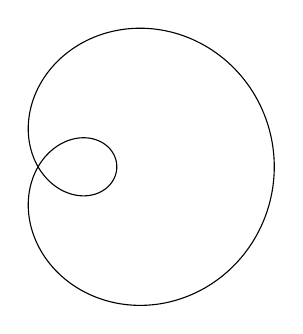
\begin{tikzpicture}
\begin{axis}[
x= 1 cm, y=1 cm,
 hide axis,
  xmin=-1,xmax=4,ymin=-2,ymax=2,
  xtick={0},
  ytick={0}]
\addplot[domain=0:360,samples=300,data cs=polar] (x,{1 + 2*cos(x)});
\end{axis}
\end{tikzpicture}
	\end{center}
Jika $a=b$, maka terbentuk kardioida berikut
\begin{center}
	\begin{tikzpicture}
\begin{axis}[
x= 1.5 cm, y=1.5 cm,
 hide axis,
  xmin=-1,xmax=4,ymin=-2,ymax=2,
  xtick={0},
  ytick={0}]
\addplot[domain=0:360,samples=300,data cs=polar] (x,{1 + cos(x)});
\end{axis}
\end{tikzpicture}
	\end{center}
Jika $b<a<2b$, maka terbentuk limacons cekung berikut
\begin{center}
	\begin{tikzpicture}
\begin{axis}[
x= 1.2 cm, y=1.2 cm,
 hide axis,
  xmin=-1,xmax=4,ymin=-2,ymax=2,
  xtick={0},
  ytick={0}]
\addplot[domain=0:360,samples=300,data cs=polar] (x,{1.2 + cos(x)});
\end{axis}
\end{tikzpicture}
	\end{center}
Jika $a\geq 2b$, maka terbentuk limacons cembung berikut
\begin{center}
	\begin{tikzpicture}
\begin{axis}[
x= 1 cm, y=1 cm,
 hide axis,
  xmin=-1,xmax=4,ymin=-2,ymax=2,
  xtick={0},
  ytick={0}]
\addplot[domain=0:360,samples=300,data cs=polar] (x,{1.6 + 0.8*cos(x)});
\end{axis}
\end{tikzpicture}
	\end{center} 
Lemniscate memiliki persamaan 
$$ r^2=\pm a^2\cos 2\theta \qquad \text{atau}\qquad r^2=\pm a^2\sin 2\theta $$
merupakan kurva yang berbentuk baling-baling sebagai berikut 
\begin{center}
	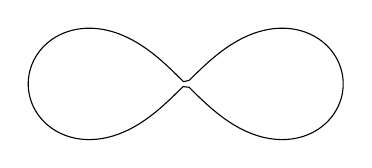
\begin{tikzpicture}
\begin{axis}[
x= 1 cm, y=1 cm,
 hide axis,
  xmin=-4,xmax=4,ymin=-2,ymax=2,
  xtick={0},
  ytick={0}]
\addplot[domain=0:360,samples=10000,data cs=polar] (x,2*sqrt{cos(2*x)});
\end{axis}
\end{tikzpicture}
	\end{center}
Posisi relatif ke sumbu kutub bergantung pada tanda di depan $a^2$ dan apakah $\sin 2\theta$ atau $\cos 2\theta$ yang muncul dalam persamaan.\\
Spiral memiliki persamaan bentuk 
$$ r=a\theta \quad (\theta\leq 0) $$
dengan kurva berikut
\begin{center}
	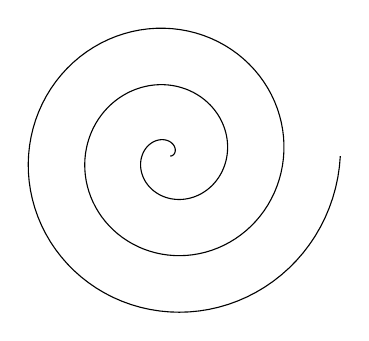
\begin{tikzpicture}
\begin{axis}[
x= 1 cm, y=1 cm,
 hide axis,
  xmin=-4,xmax=4,ymin=-2,ymax=2,
  xtick={0},
  ytick={0}]
\addplot[domain=0:360*3,samples=300,data cs=polar] (x,0.002*x);
\end{axis}
\end{tikzpicture}
	\end{center} 
Kurva rose yang memiliki persamaan 
$$ r=a\sin n\theta \qquad\text{atau}\qquad r=a\cos n\theta $$
berbentuk sebagai berikut 
\begin{center}
	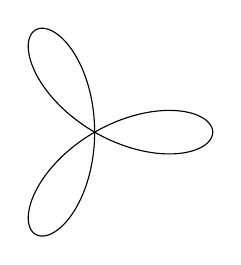
\begin{tikzpicture}
\begin{axis}[
x= 1.5 cm, y=1.5 cm,
 hide axis,
  xmin=-1,xmax=4,ymin=-2,ymax=2,
  xtick={0},
  ytick={0}]
\addplot[domain=0:360,samples=300,data cs=polar] (x,{cos(3*x)});
\end{axis}
\end{tikzpicture}
	\end{center}
Kurva ini memiliki $n$ daun jika $n$ ganjil dan $2n$ daun jika $n$ genap
\subsection{Luas dalam Koordinat Kutub}
Jika $r=f(\theta)$ kontinu dan tak negatif untuk $\alpha \leq \theta\leq \beta$ dan $0\leq \beta-\alpha\leq 2\pi$, maka luas kurvanya 
$$ A=\int_\alpha^\beta \dfrac{1}{2}[f(\theta)]^2\, d\theta = \int_\alpha^\beta \dfrac{1}{2} r^2 d\theta $$
\subsection{Volume Benda Putar dalam Koordinat Kutub}
Volume benda putar yang diputar terhadap sumbu$-x$ dan dibatasi oleh $\theta_1=\alpha$ dan $\theta_2=\beta$ adalah 
$$ V=\int_\alpha^\beta \dfrac{2}{3}\pi r^3\sin\theta \, d\theta $$
Volume benda putar yang diputar terhadap sumbu$-y$ dan dibatasi oleh $\theta_1=\alpha$ dan $\theta_2=\beta$ adalah 
$$ V=\int_\alpha^\beta \dfrac{2}{3}\pi r^3\cos\theta \, d\theta $$
\subsection{Turunan Persamaan Kurva Kutub}
Jika $r=f(\theta)$, maka 
$$ \dfrac{dy}{dx} = \dfrac{\frac{dy}{d\theta}}{\frac{dx}{d\theta}} = \dfrac{r\cos\theta +\sin\theta \frac{dr}{d\theta}}{-r\sin\theta+\cos\theta \frac{dr}{d\theta}} $$
\subsection{Panjang Busur Kurva Kutub}
Jika kurva $r=f(\theta)$ ditelusuri tepat sekali untuk $\theta$ bertambah dari $\alpha$ ke $\beta$ dan $\dfrac{dr}{d\theta}$ kontinu untuk $\alpha\leq \theta\leq \beta$, maka panjang busur kurva
$$ S=\int_\alpha^\beta \sqrt{r^2+\left(\dfrac{dr}{d\theta}\right)^2}\, d\theta $$
\subsection{Latihan Soal}
\begin{enumerate}
	\item \begin{enumerate}
		\item Buatlah sketsa kurva dari persamaan parametrik 
		$$ x=1+\cos t, ~~ y=3-\sin t, ~~ 0\leq t\leq 2\pi $$
		\item Dapatkan panjang busur dari kurva tersebut.
		\item Dapatkan semua nilai parameter $t$ yang menyebabkan kurva tersebut mempunyai garis singgung vertikal 
	\end{enumerate}
	\textbf{Penyelesaian:}
	\begin{enumerate}
		\item Tinjau bahwa $\cos t=x-1$ dan $\sin t=3-y$ sehingga $\cos^2 t+\sin^2 t =1=(x-1)^2+(3-y)^2$ \\Diperoleh persamaan lingkaran yang berpusat di $(1,3)$ dan berjari-jari 1. Karena $0\leq t\leq 2\pi$, maka kurvanya merupakan satu lingkaran penuh sebagai berikut
		\begin{center}
	\begin{tikzpicture}
\begin{axis}[
x= 1 cm, y=1 cm,
 axis lines=middle,
  xmin=-0.5,xmax=3,ymin=-0.5,ymax=4.2,
  xtick distance=1,
  ytick distance=1,
  xlabel=$x$,
  ylabel=$y$]
\draw (1,3) circle[radius=1 cm];
\end{axis}
\end{tikzpicture}
	\end{center}
	\item Karena kurvanya merupakan satu lingkaran penuh dengan jari-jari 1, maka panjang busurnya adalah keliling lingkaran yaitu $2\pi r=2\pi$\\
	Dapat dihitung pula dengan rumus panjang busur untuk kurva parametrik, yaitu 
	$$ S=\int_a^b \sqrt{\left(\dfrac{dx}{dt}\right)^2+\left(\dfrac{dy}{dt}\right)^2}\, dt $$ 
	Tinjau 
	$$ \dfrac{dx}{dt} = -\sin t \text{   dan   } \dfrac{dy}{dt}=-\cos t $$
	serta $a=0$ dan $b=2\pi$ sehingga 
	\begin{align*}
	S &= \int_0^{2\pi}\sqrt{(-\sin t)^2+(-\cos t)^2}\, dt\\
	&= \int_0^{2\pi}\, dt\\
	&= t\big|_0^{2\pi}\\
	&= 2\pi 
	\end{align*}
	\item Kurva tersebut mempunyai garis singgung vertikal jika $\dfrac{dx}{dt}=0$ dan $\dfrac{dy}{dt}\neq 0$, yaitu saat $t=0$, $t=\pi$, dan $t=2\pi$
	\end{enumerate}
	\item Dapatkan panjang busur dari kurva $r=a\cos \theta+b\sin\theta$. (Berikan gambar sketsa kurvanya).\\
	Perhatikan: bilangan $b$ dan $a$ dalam soal ini adalah dua digit terakhir NRP anda. Misalkan NRP anda adalah 06111940000076 maka $b=7$ dan $a=6$, jika $a$ atau $b$ adalah 0 ganti dengan angka 10.\\
	\textbf{Penyelesaian:}\\
	Ingat rumus panjang busur untuk kurva kutub $r=f(\theta)$ jika kurvanya ditelusuri keseluruhan satu kali untuk $\theta$ bergerak dari $\theta=\alpha$ ke $\theta=\beta$ adalah 
	$$ \int_{\alpha}^{\beta}\sqrt{r^2+\left(\dfrac{dr}{d\theta}\right)^2} \, d\theta $$
	Perhatikan bahwa
	\begin{align*}
	r^2 + \left(\dfrac{dr}{d\theta}\right)^2 &= ( a\cos \theta+b\sin\theta)^2+(-a\sin \theta+b\cos\theta)^2\\
	&= a^2\cos^2 \theta+2ab\cos\theta\sin\theta+b^2\sin^2\theta+a^2\sin^2\theta-2ab\sin\theta\cos\theta+b^2\cos^2\theta\\
	&= a^2+b^2
	\end{align*}
	Tinjau bahwa kurva tersebut ditelusuri keseluruhan satu kali untuk $\theta$ bergerak dari $\theta=0$ ke $\theta=\pi$, karena titik $(a,0)$ dan titik $(-a,\pi)$ merupakan titik yang sama dalam koordinat kutub. Jadi diperoleh 
	\begin{align*}
	S &= \int_0^\pi \sqrt{a^2+b^2}\, d\theta\\
	&= \theta\sqrt{a^2+b^2}\big|^\pi_0\\
	&= \pi\sqrt{a^2+b^2} 
	\end{align*}
	Untuk menggambar kurvanya, ingat bahwa $\dfrac{x}{r}=\cos \theta$ dan $\dfrac{y}{r}=\sin \theta$, serta $x^2+y^2=r^2$ sehingga
	\begin{align*}
	r &= a\cos\theta+b\sin\theta\\
	r &= \dfrac{ax}{r}+\dfrac{by}{r}\\
	r^2 &= ax+by\\
	x^2+y^2-ax-by &= 0 \\
	\left(x-\frac{a}{2}\right)^2+\left(y-\frac{b}{2}\right)^2 -\dfrac{a^2}{4}-\dfrac{b^2}{4} &= 0\\
	\left(x-\frac{a}{2}\right)^2+\left(y-\frac{b}{2}\right)^2 &= \dfrac{a^2+b^2}{4}
	\end{align*}
	Jadi kurvanya merupakan lingkaran yang berpusat di $\left(\frac{a}{2},\frac{b}{2}\right)$ dan berjari-jari $\frac{\sqrt{a^2+b^2}}{2}$\\
	Jika $a=6$ dan $b=7$, maka lingkarannya berpusat di $(3,3.5)$ dan berjari-jari $\frac{\sqrt{85}}{2}$, serta memotong titik $(0,0),(6,0),$ dan $(0,7)$ sebagai berikut
	\begin{center}
	\begin{tikzpicture}
\begin{axis}[
x= 0.7 cm, y=0.7 cm,
 axis lines=middle,
  xmin=-1.8,xmax=8,ymin=-1.5,ymax=9,
  xtick={0,3,6},
  ytick={0,7},
  xlabel=$x$,
  ylabel=$y$]
\draw (3,3.5) circle[radius=0.7*4.60977 cm];
\end{axis}
\end{tikzpicture}
	\end{center}
	Cara lain untuk mendapatkan panjang busurnya adalah menghitung keliling lingkaran tersebut yang berjari-jari $r=\frac{\sqrt{a^2+b^2}}{2}$, yaitu $S=2\pi r=2\pi\frac{\sqrt{a^2+b^2}}{2}=\pi\sqrt{a^2+b^2}$
	\item Diberikan partikel bergerak sepanjang kurva $\begin{cases}x=1-t\\ y=\sqrt{8+2t-t^2}\end{cases}$ dengan $-2\leq t\leq 1$
	\begin{enumerate}
		\item Nyatakan dalam persamaan kutub $r=f(\theta)$ dengan lintasan $\theta$
		\item Tentukan panjang lintasan kurva tersebut
		\item Sketsa persamaan kurva tersebut dan arah lintasannya 
	\end{enumerate}
	\textbf{Penyelesaian:}
	\begin{enumerate}
		\item Perhatikan bahwa $t=1-x$ sehingga
		\begin{align*}
		y&=\sqrt{8+2(1-x)-(1-x)^2}\\
		&=\sqrt{8+2-2x-1+2x-x^2}\\
		&= \sqrt{9-x^2}
		\end{align*}
		Ingat bahwa $y=r\sin\theta$ dan $x=r\cos\theta$ sehingga
		\begin{align*}
		r\sin\theta &=\sqrt{9-r^2\cos^2\theta}\\
		r^2\sin^2\theta &= 9-r^2\cos^2\theta\\
		r^2 &= 9
		\end{align*}
		Dapat diambil $r=f(\theta)=3$. Untuk $t=-2$, maka $x=r\cos\theta=3$ sehingga $\theta=0$, dan untuk $t=1$, maka $x=r\cos\theta=0$ sehingga $\theta=\dfrac{\pi}{2}$. Jadi $r=f(\theta)=3$ dengan $0\leq \theta\leq\dfrac{\pi}{2}$
		\item Tinjau bahwa $r=3$ dengan $0\leq \theta\leq \dfrac{\pi}{2}$ merupakan seperempat lingkaran dengan jari-jari $r=3$ di kuadran pertama, sehingga panjang lintasan kurva tersebut merupakan seperempat keliling lingkaran yaitu $\dfrac{1}{4}\cdot 2\pi r=\dfrac{3}{2}\pi$
		\item Dari jawaban (b) sudah diperoleh bentuk kurvanya.\\
		Sedangkan untuk arah lintasannya, tinjau bahwa $x$ berkurang dan $y$ bertambah ketika $t$ bergerak dari $-2$ ke 1, sehingga arahnya berlawanan arah jarum jam. Berikut sketsanya
		\begin{center}
	\begin{tikzpicture}
\begin{axis}[
x= 1.4 cm, y=1.4 cm,
 axis lines=middle,
  xmin=-0.5,xmax=3.5,ymin=-0.5,ymax=3.5,
  xtick distance=1,
  ytick distance=1,
  xlabel=$x$,
  ylabel=$y$]
\addplot[domain=0:90,samples=300,data cs=polar] (x,{3});
\end{axis}
\end{tikzpicture}
	\end{center}
	\end{enumerate}
	\item Gambarkan dan dapatkan luas irisan dari $r=\sin 2\theta$ dan $r=\cos \theta$\\
	\textbf{Penyelesaian:}\\
	Perhatikan bahwa $r_1=\sin 2\theta$ merupakan kurva rose dengan $n$ genap sehingga memiliki 4 daun sebagai berikut
	\begin{center}
	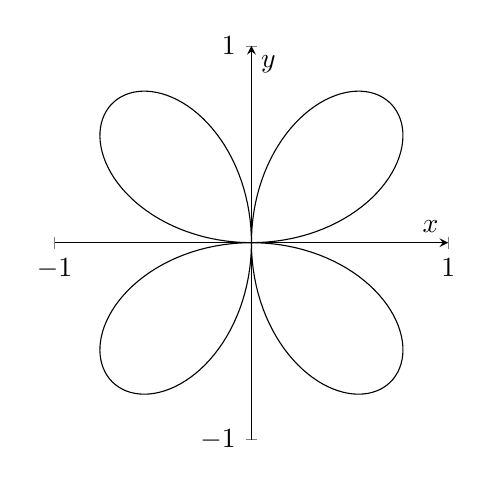
\begin{tikzpicture}
\begin{axis}[
x= 2.5 cm, y=2.5 cm,
 axis lines=middle,
  xmin=-1,xmax=1,ymin=-1,ymax=1,
  xtick distance=1,
  ytick distance=1,
  xlabel=$x$,
  ylabel=$y$]
\addplot[domain=0:360,samples=300,data cs=polar] (x,{sin(2*x)});
\end{axis}
\end{tikzpicture}
	\end{center}
	Sedangkan $r=\cos \theta$ merupakan lingkaran yang berpusat di $(0.5,0)$ dan berjari-jari $0.5$ sebagai berikut
	\begin{center}
	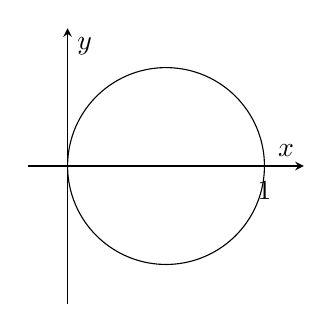
\begin{tikzpicture}
\begin{axis}[
x= 2.5 cm, y=2.5 cm,
 axis lines=middle,
  xmin=-0.2,xmax=1.2,ymin=-0.7,ymax=0.7,
  xtick distance=1,
  ytick distance=1,
  xlabel=$x$,
  ylabel=$y$]
\addplot[domain=0:360,samples=5000,data cs=polar] (x,{cos(x)});
\end{axis}
\end{tikzpicture}
	\end{center}
	Dapat diperoleh irisannya sebagai berikut 
	\begin{center}
	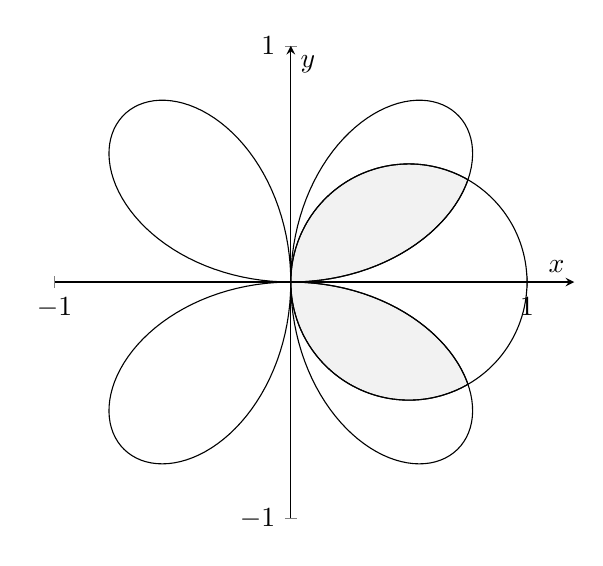
\begin{tikzpicture}
\begin{axis}[
x= 3 cm, y=3 cm,
 axis lines=middle,
  xmin=-1,xmax=1.2,ymin=-1,ymax=1,
  xtick distance=1,
  ytick distance=1,
  xlabel=$x$,
  ylabel=$y$]
\addplot[domain=0:360,samples=5000,data cs=polar] (x,{cos(x)});
\addplot[domain=0:360,samples=300,data cs=polar] (x,{sin(2*x)});
\addplot[domain=30:90,name path = B,samples=300,data cs=polar] (x,{cos(x)});
\addplot[domain=0:30,name path = A,samples=300,data cs=polar] (x,{sin(2*x)});
\addplot[domain=270:330,name path = C,samples=300,data cs=polar] (x,{cos(x)});
\addplot[domain=150:180,name path = D,samples=300,data cs=polar] (x,{sin(2*x)});
\addplot[gray,opacity=0.1] fill between[of=B and A];
\addplot[gray,opacity=0.1] fill between[of=C and D];
\end{axis}
\end{tikzpicture}
	\end{center}
	Perhatikan bahwa kurvanya simetris sehingga cukup hitung luas pada kuadran I kemudian kalikan 2. Tinjau titik perpotongan pada kuadran I adalah 
	\begin{align*}
	r_1 &= r_2\\
	\sin 2\theta &=\cos \theta\\
	2\sin \theta \cos \theta -\cos\theta &= 0\\
	\cos\theta(2\sin\theta -1) &=0
	\end{align*}
	Diperoleh perpotongannya ketika $\cos\theta=0$ yaitu $\theta_2=\dfrac{\pi}{2}$ untuk $r_2=\cos \theta$ dan $\theta_1=0$ untuk $r_1=\sin 2\theta$. Ketika $\sin\theta = \dfrac{1}{2}$, maka $\theta_1=\theta_2=\dfrac{\pi}{6}$. Jadi, luas irisan kurva pada kuadran I dapat dirumuskan
	\begin{align*}
	L &= \int_0^\frac{\pi}{6} \dfrac{1}{2} r_1^2 \, d\theta + \int_\frac{\pi}{6}^\frac{\pi}{2}\dfrac{1}{2}r_2^2 \, d\theta\\
	&= \dfrac{1}{2} \int_0^\frac{\pi}{6} \sin^2 2\theta \, d\theta + \dfrac{1}{2} \int_\frac{\pi}{6}^\frac{\pi}{2} \cos^2\theta \, d\theta \\
	&= \dfrac{1}{2} \int_0^\frac{\pi}{6} \dfrac{1-\cos 4\theta}{2}\, d\theta + \dfrac{1}{2} \int_\frac{\pi}{6}^\frac{\pi}{2} \dfrac{1+\cos 2\theta}{2}\, d\theta \\
	&= \dfrac{1}{4}\left[\theta -\dfrac{\sin 4\theta}{4}\right]_0^\frac{\pi}{6} + \dfrac{1}{4}\left[\theta+\dfrac{\sin 2\theta}{2}\right]_\frac{\pi}{6}^\frac{\pi}{2}\\
	&= \dfrac{1}{4}\left[\dfrac{\pi}{6}-\dfrac{1}{8}\sqrt{3}+\dfrac{\pi}{2}+0-\dfrac{\pi}{6}-\dfrac{1}{4}\sqrt{3}\right]\\
	&= \dfrac{\pi}{8}-\dfrac{3}{32}\sqrt{3}
	\end{align*}
	Jadi luas total irisan adalah $2L=\dfrac{\pi}{4}-\dfrac{3}{16}\sqrt{3}$
	\item Dapatkan kemiringan garis singgung pada kurva $r=3\sin 3\theta$ di $\theta=\dfrac{\pi}{4}$\\
	\textbf{Penyelesaian:}\\
	Ingat bahwa kemiringan garis singgung kurva di suatu titik merupakan turunan persamaan kurva tersebut di titik itu, dan turunan persamaan kurva kutub adalah
	$$ \dfrac{dy}{dx} = \dfrac{\frac{dy}{d\theta}}{\frac{dx}{d\theta}} = \dfrac{r\cos\theta +\sin\theta \frac{dr}{d\theta}}{-r\sin\theta+\cos\theta \frac{dr}{d\theta}} $$
	sehingga diperoleh 
	\begin{align*}
	\dfrac{dy}{dx} &= \dfrac{3\sin 3\theta \cos \theta+\sin \theta (9\cos 3\theta)}{-3\sin 3\theta\sin\theta +\cos\theta (9\cos 3\theta)}
	\end{align*}
	Untuk $\theta=\dfrac{\pi}{4}$, maka 
	\begin{align*}
	\dfrac{dy}{dx} &= \dfrac{3\left( \frac{1}{2}\sqrt{2}\right)\left( \frac{1}{2}\sqrt{2}\right)+9\left( \frac{1}{2}\sqrt{2}\right) \left(-\frac{1}{2}\sqrt{2}\right)}{-3\left(\frac{1}{2}\sqrt{2}\right)\left(\frac{1}{2}\sqrt{2}\right)+9\left(\frac{1}{2}\sqrt{2}\right)\left(-\frac{1}{2}\sqrt{2}\right)}\\
	&= \dfrac{\frac{3}{2}-\frac{9}{2}}{-\frac{3}{2}-\frac{9}{2}}\\
	&= \dfrac{-3}{-6} = \dfrac{1}{2}
	\end{align*}
	Jadi kemiringan garis singgung pada kurva $r=3\sin 3\theta$ di $\theta=\dfrac{\pi}{4}$ adalah $\dfrac{1}{2}$
\end{enumerate}
\newpage
\section{Bab 6}
\subsection{Barisan Tak Hingga}
Barisan tak hingga $a_1,a_2,a_3,\cdots$ dapat dituliskan dalam notasi kurung $\{a_n\}_{n=1}^\infty$ atau $\{a_n\}$\\
Barisan $\{a_n\}$ disebut konvergen ke $L$ jika $\displaystyle \lim_{n\rightarrow +\infty} a_n = L$ dengan $-\infty<L<\infty$
\subsection{Sifat-Sifat Barisan Konvergen}
Diberikan barisan $\{a_n\}$ dan $\{b_n\}$ yang masing-masing konvergen ke limit $L_1$ dan $L_2$ dan $c$ adalah suatu konstanta, maka
\begin{enumerate}
	\item $\displaystyle \lim_{n\rightarrow +\infty} c = c$
	\item $\displaystyle \lim_{n\rightarrow +\infty} ca_n = c\lim_{n\rightarrow +\infty} a_n = cL_1$
	\item $\displaystyle \lim_{n\rightarrow +\infty} (a_n\pm b_n) = \lim_{n\rightarrow +\infty} a_n \pm \lim_{n\rightarrow +\infty} b_n = L_1\pm L_2$
	\item $\displaystyle \lim_{n\rightarrow +\infty} (a_n\cdot b_n) = \lim_{n\rightarrow +\infty} a_n \cdot \lim_{n\rightarrow +\infty} b_n = L_1L_2$
	\item $\displaystyle \lim_{n\rightarrow +\infty} \left(\dfrac{a_n}{b_n}\right) = \dfrac{\displaystyle\lim_{n\rightarrow +\infty} a_n}{\displaystyle\lim_{n\rightarrow +\infty} b_n} = \dfrac{L_1}{L_2}$, ~~jika $L_2\neq 0$
\end{enumerate}
Jika barisan $\{a_n\}$ dan $\{c_n\}$ masing-masing konvergen ke $L$ dan $a_n\leq b_n\leq c_n$ untuk $n\geq K$ ($K$ bilangan bulat tertentu), maka $\{b_n\}$ juga konvergen ke $L$
\subsection{Barisan Monoton}
Suatu barisan $\{a_n\}$ disebut naik jika $a_1<a_2<a_3<\cdots <a_n<\cdots$\\
Suatu barisan $\{a_n\}$ disebut turun jika $a_1>a_2>a_3>\cdots >a_n>\cdots$\\
Suatu barisan $\{a_n\}$ disebut tidak naik jika $a_1\geq a_2\geq a_3\geq \cdots \geq a_n\geq \cdots$\\
Suatu barisan $\{a_n\}$ disebut tidak turun jika $a_1\leq a_2\leq a_3\leq \cdots \leq a_n\leq \cdots$\\
Secara umum, untuk semua pasangan suku-suku yang berurutan $a_n$ dan $a_{n+1}$\\
Jika $a_{n+1}-a_n>0$ maka disebut barisan naik\\
Jika $a_{n+1}-a_n<0$ maka disebut barisan turun\\
Jika $a_{n+1}-a_n\leq 0$ maka disebut barisan tidak naik \\
Jika $a_{n+1}-a_n\geq 0$ maka merupakan barisan tidak turun\\
Jika semua suku pada barisan tersebut positif, maka \\
Barisan monoton naik jika $a_{n+1}/a_n>1$\\
Barisan monoton turun jika $a_{n+1}/a_n<1$\\
Barisan monoton tidak naik jika $a_{n+1}/a_n\leq 1$\\
Barisan monoton tidak turun jika $a_{n+1}/a_n\geq 1$
\subsection{Deret Tak Hingga}
Deret tak hingga adalah suatu ekspresi yang dapat ditulis dalam bentuk 
$$ \sum_{k=1}^\infty u_k = u_1+u_2+u_3+\cdots+u_k+\cdots $$
Bilangan-bilangan $u_1,u_2,u_3,\cdots$ disebut suku-suku dari deret tersebut.\\
Misalkan $\{s_n\}$ adalah barisan dari jumlahan parsial deret $u_1+u_2+\cdots+u_k+\cdots$. Jika barisan $\{s_n\}$ konvergen ke suatu limit $S$, maka deret tersebut konvergen dan $S$ adalah jumlah dari deret tersebut, dapat ditulis 
$$ S=\sum_{k=1}^\infty u_k $$
Jika barisan dari jumlahan parsial tersebut divergen, maka deret tersebut divergen dan tidak mempunyai jumlah.\\
Deret geometri tak hingga 
$$ \sum_{k=0}^\infty ar^k = a+ar+ar^2+ar^3+\cdots + ar^{k-1}+\cdots \qquad (a\neq 0) $$
konvergen jika $|r|<1$ dan divergen jika $|r|\geq 1$. Jika deret konvergen, maka jumlah deret adalah 
$$ \sum_{k=0}^\infty ar^k =  \dfrac{a}{1-r} $$
Deret harmonik merupakan deret divergen dengan bentuk 
$$ \sum_{k=1}^\infty \dfrac{1}{k} = 1+\dfrac{1}{2}+\dfrac{1}{3}+\dfrac{1}{4}+\dfrac{1}{5}+\cdots  $$
Deret$-p$ atau deret hyperharmonic merupakan deret dengan bentuk 
$$ \sum_{k=1}^\infty \dfrac{1}{k^p} = 1+\dfrac{1}{2^p}+\dfrac{1}{3^p}+\dfrac{1}{4^p}+\dfrac{1}{5^p}+\cdots  $$
yang konvergen jika $p>1$ dan divergen jika $0<p\leq 1$
\subsection{Sifat-Sifat Aljabar Deret Tak Hingga}
\begin{enumerate}
	\item Jika $\displaystyle \sum_{k=1}^\infty u_k$ dan $\displaystyle \sum_{k=1}^\infty v_k$ deret konvergen, maka $\displaystyle \sum_{k=1}^\infty (u_k\pm v_k)$ juga konvergen dengan jumlah 
$$ \sum_{k=1}^\infty (u_k\pm v_k) = \sum_{k=1}^\infty u_k \pm \sum_{k=1}^\infty v_k $$
	\item Jika $c$ adalah konstanta tak nol, maka deret $\displaystyle \sum_{k=1}^\infty u_k$ dan $\displaystyle \sum_{k=1}^\infty cu_k$ keduanya konvergen atau keduanya divergen. Jika deretnya konvergen, maka jumlahnya
$$ \sum_{k=1}^\infty cu_k = c \sum_{k=1}^\infty u_k   $$
\item Penghapusan sejumlah berhingga suku-suku pada suatu deret tidak memengaruhi konvergensi dan divergensi dari deret tersebut
\end{enumerate}
\subsection{Uji Integral}
Misalkan $\displaystyle \sum_{k=1}^\infty u_k$ adalah deret dengan suku-suku positif dan $f(x)$ merupakan fungsi yang dihasilkan jika $k$ diganti $x$ dalam rumus $u_k$. Jika $f$ adalah deret turun dan kontinu pada interval $[a,+\infty)$, maka 
$$ \sum_{k=a}^\infty u_k \qquad\text{dan}\qquad \int_a^{+\infty} f(x)\, dx $$
keduanya konvergen atau keduanya divergen. 
\subsection{Uji Rasio}
Jika diberikan deret $\displaystyle \sum_{k=1}^\infty u_k$ dengan suku-suku positif dan dimisalkan bahwa $\displaystyle \rho = \lim_{k\rightarrow +\infty} \dfrac{u_{k+1}}{u_k}$, maka 
\begin{enumerate}
	\item Deret konvergen jika $\rho<1$
	\item Deret divergen jika $\rho>1$
	\item Deret mungkin konvergen atau divergen jika $\rho=1$ sehingga diperlukan uji yang lain
\end{enumerate}
\subsection{Prinsip Informal}
\begin{enumerate}
	\item Prinsip Informal I: Suku-suku konstan dalam penyebut $u_k$ dapat dihilangkan tanpa berpengaruh pada konvergensi maupun divergensi deret
	\item Prinsip Informal II: Jika sebuah polinomial dalam $k$ tampak sebagai faktor pembilang atau penyebut dari $u_k$, maka semua suku (kecuali $k$ dengan pangkat tertinggi) pada polinomial dapat dihilangkan tanpa memengaruhi konvergensi maupun divergensi deret.
\end{enumerate}
\subsection{Uji Deret Berganti Tanda}
Suatu deret berganti tanda dengan bentuk 
$$ \sum_{k=1}^\infty (-1)^k a_k = -a_1+a_2-a_3+a_4-\cdots $$
atau 
$$ \sum_{k=1}^\infty (-1)^{k+1} a_k = a_1-a_2+a_3-a_4+\cdots $$
dan diasumsikan $a_k$ positif merupakan deret yang konvergen jika kedua kondisi berikut terpenuhi
\begin{enumerate}
	\item $a_1>a_2>a_3>\cdots >a_k>\cdots$
	\item $\displaystyle \lim_{k\rightarrow +\infty} a_k = 0$
\end{enumerate}
\subsection{Deret Pangkat}
Deret pangkat memiliki bentuk 
$$ \sum_{n=0}^{+\infty} a_n(x-c)^n = a_0+a_1(x-c)+a_2(x-c)^2+a_3(x-c)^3+\cdots $$
yang dapat dipastikan konvergen untuk $x=c$ karena 
$$ \sum_{n=0}^{+\infty} a_n(x-c)^n = 0 $$
\subsection{Deret Taylor dan Maclaurin}
Jika $f(x)$ memiliki turunan pada semua tingkat di $x=a$, maka deret Taylor untuk $f(x)$ di sekitar $x=a$ menjadi
$$ \sum_{k=0}^\infty \dfrac{f^{(k)}(a)}{k!} (x-a)^k = f(a)+f'(a)(x-a)+\dfrac{f''(a)}{2!}(x-a)^2+\cdots +\dfrac{f^{(k)}(a)}{k!}(x-a)^k +\cdots $$
Pada kasus khusus yaitu $a=0$, deret Taylor tersebut disebut deret Maclaurin untuk $f(x)$ yang memiliki bentuk
$$ \sum_{k=0}^\infty \dfrac{f^{(k)}(0)}{k!} x^k = f(0)+f'(0)(x)+\dfrac{f''(0)}{2!}x^2+\cdots +\dfrac{f^{(k)}(0)}{k!}x^k+\cdots $$
Berikut dua deret Maclaurin yang paling umum dijumpai
\begin{enumerate}
	\item Deret Maclaurin
	$$ \dfrac{1}{1-x} = \sum_{k=0}^\infty x^k = 1+x+x^2+x^3+\cdots $$
	memiliki selang konvergensi $-1<x<1$
	\item Deret Maclaurin
	$$ e^x = \sum_{k=0}^\infty \dfrac{x^k}{k!} = 1+x+\dfrac{x^2}{2!}+\dfrac{x^3}{3!} + \cdots $$
	memiliki selang konvergensi seluruh bilangan real
\end{enumerate}
\subsection{Turunan dan Integral Deret Pangkat}
Jika suatu fungsi $f(x)$ direpresentasikan oleh suatu deret pangkat misal
$$ f(x) = \sum_{k=0}^\infty c_k(x-a)^k $$
dengan jari-jari konvergensi $R$, maka 
\begin{enumerate}
	\item Deret-deret suku diferensialnya 
	$$ \sum_{k=0}^\infty \dfrac{d}{dx} [c_k(x-a)^k] = \sum_{k=0}^\infty kc_k (x-a)^{k-1} $$
	memiliki jari-jari konvergensi $R$
	\item Fungsi $f(x)$ diferensiabel pada selang $(a-R,a+R)$ dan untuk setiap $x$ dalam selang ini 
	$$ f'(x) = \sum_{k=0}^\infty \dfrac{d}{dx} [c_k(x-a)^k] = \sum_{k=0}^\infty kc_k(x-a)^{k-1} $$
	\item Deret-deret suku integrasinya 
	$$ \sum_{k=0}^\infty \left[\int c_k(x-a)^k \, dx\right] = \sum_{k=0}^\infty \dfrac{c_k}{k+1} (x-a)^{k+1} $$
	memiliki jari-jari konvergensi $R$
	\item Fungsi $f(x)$ kontinu pada selang $(a-R,a+R)$ dan untuk setiap $x$ dalam selang ini
	$$ \int f(x)\, dx = \sum_{k=0}^\infty \left[\int c_k(x-a)^k \, dx\right] +C $$
	\item Untuk setiap $\alpha$ dan $\beta$ dalam selang $(a-R,a+R)$, maka
	$$ \int_\alpha^\beta f(x)\, dx = \sum_{k=0}^\infty \left[\int_\alpha^\beta c_k(x-a)^k \, dx\right]$$ 
\end{enumerate}
\subsection{Latihan Soal}
\begin{enumerate}
	\item \begin{enumerate}
		\item Gunakan uji yang sesuai untuk menentukan apakah deret
	$$ \sum_{n=1}^\infty \dfrac{4}{3^n+1} \text{ konvergen atau divergen} $$
		\item Dapatkan jumlahan deret 
		$$ \sum_{k=1}^\infty \left[\dfrac{7}{3^k}+\dfrac{6}{(k+3)(k+4)}\right] $$
	\end{enumerate}
	\textbf{Penyelesaian:}
	\begin{enumerate}
		\item Dengan Prinsip Informal I, suku konstan yaitu 1 pada penyebut dapat dihilangkan tanpa memengaruhi konvergensi deret tersebut, sehingga bentuknya menjadi 
		$$ \sum_{n=1}^\infty \dfrac{4}{3^n} $$
		Bentuk tersebut merupakan deret geometri tak hingga dengan $a=\dfrac{4}{3}$ dan $r=\dfrac{1}{3}$ yang jelas konvergen.
		\item Tinjau bahwa 
		$$ \sum_{k=1}^\infty \left[\dfrac{7}{3^k}+\dfrac{6}{(k+3)(k+4)}\right] = \sum_{k=1}^\infty \dfrac{7}{3^k}+\sum_{k=1}^\infty \dfrac{6}{(k+3)(k+4)}  $$
		Perhatikan bahwa $\displaystyle \sum_{k=1}^\infty \dfrac{7}{3^k} $ merupakan deret geometri tak hingga dengan $a=\dfrac{7}{3}$ dan $r=\dfrac{1}{3}$ sehingga 
		$$ \sum_{k=1}^\infty \dfrac{7}{3^k} = \dfrac{a}{1-r} = \dfrac{\frac{7}{3}}{1-\frac{1}{3}} = \dfrac{7}{2} $$
		Perhatikan pula $\dfrac{6}{(k+3)(k+4)}=6\left(\dfrac{1}{k+3}-\dfrac{1}{k+4}\right)$ sehingga 
		\begin{align*}
		\sum_{k=1}^\infty \dfrac{6}{(k+3)(k+4)} &= \lim_{k\rightarrow \infty} 6\bigg[\left(\dfrac{1}{4}-\dfrac{1}{5}\right)+\left(\dfrac{1}{5}-\dfrac{1}{6}\right)+\left(\dfrac{1}{6}-\dfrac{1}{7}\right)+\cdots \\
		&\qquad \qquad +\left(\dfrac{1}{k+2}-\dfrac{1}{k+3}\right)+\left(\dfrac{1}{k+3}-\dfrac{1}{k+4}\right)\bigg]\\
		&= \lim_{k\rightarrow \infty} 6 \left[\dfrac{1}{4}-\dfrac{1}{k+4}\right]\\
		&= 6\left[\dfrac{1}{4}-0\right]=\dfrac{3}{2}
		\end{align*}
		Jadi 
		$$ \sum_{k=1}^\infty \left[\dfrac{7}{3^k}+\dfrac{6}{(k+3)(k+4)}\right] =\dfrac{7}{2} + \dfrac{3}{2} = 5 $$
	\end{enumerate}
	\item Selesaikan 
	\begin{enumerate}
		\item Tentukan konvergensi barisan $\left\{ n\sin\frac{\pi}{n}\right\}^\infty_{n=1}$;\\
		Dari jawaban tersebut, tentukan konvergensi $\left\{ \dfrac{n^2}{2n+1}\sin\dfrac{\pi}{n}\right\}^\infty_{n=1}$
		\item Dengan uji perbandingan, tentukan deret berikut konvergen ataukah divergen?
		$$ \sum_{n=0}^\infty \dfrac{2^n\sin^2(5n)}{4^n+\cos^2 n} $$
	\end{enumerate}
	\textbf{Penyelesaian:}
	\begin{enumerate}
		\item Akan dicari $\displaystyle \lim_{n\rightarrow +\infty} n\sin \frac{\pi}{n}=L_1$\\ Misalkan $\dfrac{1}{n}=k$, maka $k\rightarrow 0^+$ karena $n\rightarrow +\infty$, sehingga
		$$ L_1=\lim_{k\rightarrow 0^+} \dfrac{\sin \pi k}{k} = \pi $$ 
		Jadi barisan $\left\{ n\sin\frac{\pi}{n}\right\}^\infty_{n=1}$ konvergen ke $\pi$\\
		Selanjutnya tinjau, 
		$$ \dfrac{n^2}{2n+1}\sin \frac{\pi}{n}=\dfrac{n}{2n+1}\times n\sin\frac{\pi}{n}$$ 
		Dapat diperoleh $\displaystyle \lim_{n\rightarrow +\infty} \dfrac{n}{2n+1}=\lim_{n\rightarrow +\infty} \dfrac{1}{2+\frac{1}{n}}=\dfrac{1}{2}= L_2$\\
		Akibatnya $$ \lim_{n\rightarrow +\infty} \dfrac{n^2}{2n+1}\sin \frac{\pi}{n} = \lim_{n\rightarrow +\infty} \dfrac{n}{2n+1}\cdot \lim_{n\rightarrow +\infty} n\sin \frac{\pi}{n} = L_1\cdot L_2=\dfrac{\pi}{2} $$
		Jadi barisan $\left\{ \dfrac{n^2}{2n+1}\sin\dfrac{\pi}{n}\right\}^\infty_{n=1}$ konvergen ke $\dfrac{\pi}{2}$
		\item Tinjau bahwa $0\leq \sin^2(5n)\leq 1$ sehingga $2^n\sin^2(5n)\leq 2^n$\\
		Tinjau pula $0\leq \cos^2 n\leq 1$ sehingga $4^n\leq 4^n+\cos^2 n$ dan $\dfrac{1}{4^n+\cos^2 n}\leq \dfrac{1}{4^n}$\\
		Akibatnya 
		$$ \dfrac{2^n\sin^2(5n)}{4^n+\cos^2 n} \leq \dfrac{2^n}{4^n} = \dfrac{1}{2^n} $$
		Karena $\displaystyle \sum_{n=0}^\infty \dfrac{1}{2^n}$ merupakan deret geometri tak hingga dengan $a=1$ dan $r=\dfrac{1}{2}$ yang jelas konvergen sehingga deret $\displaystyle \sum_{n=0}^\infty \dfrac{2^n\sin^2(5n)}{4^n+\cos^2 n}$ juga konvergen.
	\end{enumerate}
	\item Buktikan $\displaystyle \sum_{k=2}^\infty \dfrac{1}{k(\ln k)^p}$ konvergen jika $p>1$\\
	\textbf{Penyelesaian:}\\
	Uji konvergensi deret tersebut dengan uji integral berikut
	\begin{align*}
	\int_2^\infty \dfrac{1}{x(\ln x)^p}\, dx
	\end{align*}
	Misalkan $\ln x=u$ sehingga $\dfrac{1}{x}\, dx=du$, akan dihitung dulu integralnya tanpa menggunakan batas integral
	\begin{align*}
	\int \dfrac{1}{x(\ln x)^p}\, dx &= \int \dfrac{1}{u^p} \,du\\
	&= \int u^{-p} \, du\\
	&= \dfrac{u^{1-p}}{1-p}\\
	&= \dfrac{(\ln x)^{1-p}}{1-p}
	\end{align*}
	Dapat diperoleh 
	\begin{align*}
	\int_2^\infty \dfrac{1}{x(\ln x)^p}\, dx &= \lim_{a\rightarrow\infty} \int_2^a \dfrac{1}{x(\ln x)^p}\, dx\\
	&= \lim_{a\rightarrow\infty} \left(\dfrac{(\ln a)^{1-p}}{1-p}-\dfrac{(\ln 2)^{1-p}}{1-p}\right)\\
	&= \dfrac{1}{1-p}\left( \lim_{a\rightarrow\infty} \dfrac{1}{(\ln a)^{p-1}}-\dfrac{1}{(\ln 2)^{p-1}}\right)
	\end{align*}
	Jika $p>1$, diperoleh
	 $$\dfrac{1}{1-p}\left( \lim_{a\rightarrow\infty} \dfrac{1}{(\ln a)^{p-1}}-\dfrac{1}{(\ln 2)^{p-1}}\right) = \dfrac{1}{1-p}\left(0-\dfrac{1}{(\ln 2)^{p-1}}\right) = \dfrac{1}{(p-1)(\ln 2)^{p-1}}$$
	Dapat disimpulkan deret tersebut konvergen jika $p>1$\\
	Jika $p<1$, maka $p-1<0$ sehingga
	 $$\dfrac{1}{1-p}\left( \lim_{a\rightarrow\infty} \dfrac{1}{(\ln a)^{p-1}}-\dfrac{1}{(\ln 2)^{p-1}}\right) = \infty$$
	Dapat disimpulkan deret tersebut divergen jika $p<1$
	\item Selesaikan:
	\begin{enumerate}
		\item Diberikan $\{a_n\}^\infty_{n=1}$ dengan $a_n=\dfrac{1}{n^2}+\dfrac{3}{n^2}+\dfrac{5}{n^2}+\cdots +\dfrac{2n-1}{n^2}$\\
		Tuliskan 5 suku pertama barisan, dan dapatkan $\displaystyle \lim_{n\rightarrow \infty} a_n$
		\item Jika diberikan barisan $(a_n)=(0,1,0,1,0,1,\dots)$ dan $(b_n)=(1,0,1,0,1,0,\dots)$ maka selidiki tentang konvergensi dari: $1. (a_n+b_n);\quad 2. (a_n\cdot b_n);\quad 3. \left(\dfrac{a_n}{b_n}\right)$
	\end{enumerate}
	\textbf{Penyelesaian:}
	\begin{enumerate}
		\item Tinjau bahwa 
		$$ a_n = \dfrac{1+3+5+\cdots +2n-1}{n^2} =\dfrac{\frac{n}{2}(1+(2n-1))}{n^2}=1$$
		untuk $n=1,2,3,\cdots$. Diperoleh $(a_n)=(1,1,1,\dots)$ sehingga $a_1=a_2=a_3=a_4=a_5=1$ merupakan 5 suku pertama barisan tersebut dan $\displaystyle \lim_{n\rightarrow \infty} a_n=1$ 
		\item \begin{enumerate}
		\item Tinjau $(a_n+b_n)=(1,1,1,\dots)$ sehingga barisan tersebut konvergen ke 1
		\item Tinjau $(a_n\cdot b_n)=(0,0,0,\dots)$ sehingga barisan tersebut konvergen ke 0
		\item Tinjau untuk $n=2$, $\dfrac{a_n}{b_n}$ tidak terdefinisi sehingga konvergensi barisan $\left(\dfrac{a_n}{b_n}\right)$ tidak dapat ditentukan
		\end{enumerate}
	\end{enumerate}
	\item Diketahui fungsi $f(x)=\dfrac{1}{1-ax}$
	\begin{enumerate}
		\item Dapatkan deret Maclaurin dari $f(x)$ (Nyatakan dalam notasi sigma)
		\item Gunakan hasil dari (a) untuk mendapatkan deret Maclaurin dari fungsi $f(x)=\dfrac{1}{(1-ax)^2}$
	\end{enumerate}
	Perhatikan: bilangan $a$ dalam soal ini adalah digit terakhir NRP anda. Misalkan NRP anda adalah 06111940000076 maka $a=6$, jika $a=0$ ganti dengan angka 10.\newpage
	\textbf{Penyelesaian:}
	\begin{enumerate}
		\item Tinjau 
		\begin{multicols}{2}
		\begin{align*}
		f(x) &= \dfrac{1}{1-ax}\\
		f'(x) &= \dfrac{a}{(1-ax)^2}\\
		f''(x) &= \dfrac{a\cdot 2a}{(1-ax)^3}\\
		f'''(x) &= \dfrac{a\cdot 2a\cdot 3a}{(1-ax)^4}\\
		&~~\vdots\\
		f^{(k)}(x) &= \dfrac{a\cdot 2a\cdot 3a\cdots ka}{(1-ax)^{k+1}} = \dfrac{k!a^k}{(1-ax)^{k+1}}
		\end{align*}
		\begin{align*}
		f(0) &= 1\\
		f'(0) &= a\\
		f''(0) &= a\cdot 2a\\
		f'''(0) &= a\cdot 2a\cdot 3a\\
		&~~\vdots\\
		f^{(k)}(0) &= a\cdot 2a\cdot 3a\cdots ka=k!a^k
		\end{align*}
		\end{multicols}
		Diperoleh deret Maclaurin dari $f(x)$
		\begin{align*}
		\sum_{k=0}^\infty \dfrac{f^{(k)}(0)}{k!}x^k &= f(0) + f'(0)x +\dfrac{f''(0)}{2!}x^2+\cdots+\dfrac{f^{(k)}(0)}{k!}x^k+\cdots\\
		&= 1+(a)(x)+\dfrac{2!a^2}{2!}x^2+\cdots+\dfrac{k!a^k}{k!}x^k+\cdots\\
		&= 1+(ax)+(ax)^2+\cdots (ax)^k+\cdots\\
		&= \sum_{k=0}^\infty (ax)^k
\end{align*}				 
		Alternatif penyelesaian dengan metode substitusi.\\
		Tinjau deret Maclaurin dari $\displaystyle \dfrac{1}{1-x}=1+x+x^2+x^3+\cdots=\sum_{k=0}^\infty x^k$. Dengan metode substitusi diperoleh deret Maclaurin dari $f(x)$ adalah 
		$$ \dfrac{1}{1-ax}=1+ax+(ax)^2+(ax)^3+\cdots =\sum_{k=0}^\infty (ax)^k$$
		\item Tinjau $\dfrac{d}{dx}(ax)^k=ka(ax)^{k-1}$ sehingga
	\begin{align*}
	\dfrac{d}{dx} \left(\dfrac{1}{1-ax}\right) &= \dfrac{d}{dx} \sum_{k=0}^\infty (ax)^k\\
	\dfrac{a}{(1-ax)^2} &= \sum_{k=0}^\infty ka(ax)^{k-1}\\
	\dfrac{a}{(1-ax)^2} &= a\sum_{k=0}^\infty k(ax)^{k-1}\\
	\dfrac{1}{(1-ax)^2} &= \sum_{k=0}^\infty k(ax)^{k-1} = 1+2(ax)+3(ax)^2+\cdots 
	\end{align*}
	\end{enumerate}
\end{enumerate}

\end{document}
